% covtl-pipeline --- Dynamic Polar Visualization Manual
% SPDX-License-Identifier: GPL-3.0-or-later
% Copyright (C) 2026 Frédéric Berthommier
%
% Compile with plain pdflatex (standard packages only):
%     pdflatex polar_visualization.tex && pdflatex polar_visualization.tex
% (run twice for the table of contents and cross references)

\documentclass[11pt,a4paper]{article}

% --- Packages ---
\usepackage[T1]{fontenc}
\usepackage[utf8]{inputenc}
\usepackage{lmodern}
\usepackage{graphicx}
\usepackage{xcolor}
\usepackage{geometry}
\usepackage{amsmath}
\usepackage{amssymb}
\usepackage{booktabs}
\usepackage{tabularx}
\usepackage{enumitem}
\usepackage{longtable}
\usepackage{fancyhdr}
\usepackage{titlesec}
\usepackage{listings}
\usepackage{needspace}
\usepackage[
    colorlinks=true,
    linkcolor=blue!60!black,
    citecolor=blue!50!black,
    urlcolor=blue!70!black,
    bookmarks=true,
    bookmarksnumbered=true,
    pdftitle={covtl-pipeline Dynamic Polar Visualization},
    pdfauthor={Frederic Berthommier},
    pdfsubject={Two-branch polar figure of the COVTL articulatory trajectories},
    pdfkeywords={articulatory synthesis, polar coordinates, COVTL, superposition, VocalTractLab, visualization}
]{hyperref}

% --- Geometry ---
\geometry{a4paper, top=2.5cm, bottom=2.5cm, left=2.5cm, right=2.5cm}
\setlength{\headheight}{14pt}
\setlength{\parindent}{0pt}
\setlength{\parskip}{0.45em}

% --- Page style ---
\pagestyle{fancy}
\fancyhf{}
\fancyhead[L]{\small\itshape covtl-pipeline --- Dynamic Polar Visualization}
\fancyhead[R]{\small v1.1.0}
\fancyfoot[C]{\thepage}
\renewcommand{\headrulewidth}{0.3pt}
\renewcommand{\footrulewidth}{0pt}

% --- Section formatting (matches the main repository manual) ---
\titleformat{\section}{\Large\bfseries\color{blue!50!black}}{\thesection}{0.6em}{}
\titleformat{\subsection}{\large\bfseries\color{blue!40!black}}{\thesubsection}{0.5em}{}
\titleformat{\subsubsection}{\normalsize\bfseries}{\thesubsubsection}{0.4em}{}

% --- Listings (code blocks) ---
\definecolor{codebg}{HTML}{F5F5F5}
\definecolor{codeframe}{HTML}{CCCCCC}
\definecolor{codecomment}{HTML}{6A737D}
\definecolor{codekeyword}{HTML}{D73A49}
\definecolor{codestring}{HTML}{032F62}
\lstdefinestyle{shell}{
    backgroundcolor=\color{codebg}, frame=single,
    rulecolor=\color{codeframe},
    basicstyle=\ttfamily\footnotesize,
    commentstyle=\color{codecomment}\itshape,
    keywordstyle=\color{codekeyword}\bfseries,
    stringstyle=\color{codestring},
    showstringspaces=false, breaklines=true, breakatwhitespace=true,
    numbers=none, xleftmargin=4pt, xrightmargin=4pt,
    framexleftmargin=4pt, framexrightmargin=4pt,
    language=bash,
    morekeywords={vtl-synth, run, polar-build, polar-video, python, pip,
                  git, ffmpeg, cd, pytest}
}
\lstdefinestyle{python}{
    backgroundcolor=\color{codebg}, frame=single,
    rulecolor=\color{codeframe},
    basicstyle=\ttfamily\footnotesize,
    commentstyle=\color{codecomment}\itshape,
    keywordstyle=\color{codekeyword}\bfseries,
    stringstyle=\color{codestring},
    showstringspaces=false, breaklines=true, breakatwhitespace=true,
    numbers=none, xleftmargin=4pt, xrightmargin=4pt,
    framexleftmargin=4pt, framexrightmargin=4pt,
    language=Python
}
\lstdefinestyle{json}{
    backgroundcolor=\color{codebg}, frame=single,
    rulecolor=\color{codeframe},
    basicstyle=\ttfamily\footnotesize,
    commentstyle=\color{codecomment}\itshape,
    showstringspaces=false, breaklines=true,
    numbers=none, xleftmargin=4pt, xrightmargin=4pt,
    framexleftmargin=4pt, framexrightmargin=4pt
}

\newcommand{\code}[1]{\texttt{#1}}
\newcommand{\vbranch}{\ensuremath{z_{\mathrm{v}}(t)}}
\newcommand{\cbranch}{\ensuremath{z_{\mathrm{c}}(t)}}

\title{\textbf{The covtl-pipeline Dynamic Polar Visualization}\\[0.4em]
\large Two-branch display of the COVTL articulatory trajectories\\
(vocalic background and consonantal excursions)}
\author{Fr\'ed\'eric Berthommier}
\date{Version 1.1.0 --- September 2026}

\begin{document}

\maketitle

\begin{center}
\begin{minipage}{0.88\textwidth}
\small\emph{Scope.} This manual documents the \emph{dynamic polar
figure} of the covtl-pipeline articulatory synthesizer (module
\code{vtl\_synth/video/polar\_video.py}): the polar coordinate model
behind it, the two-branch reconstruction of the vocalic and
consonantal trajectories from the engine's own complex values, the
\code{.polar} intermediate file, and the dual-panel MP4 output. It is
one of the five manuals of the repository, a companion to the main
manual (\code{docs/manual.pdf}), the speaker-registry manual
(\code{docs/speakers.pdf}), the language-pack manual
(\code{docs/language\_pack.pdf}) and the expressive-prosody guide
(\code{docs/expressive\_prosody.pdf}).
\end{minipage}
\end{center}

\vspace{0.5em}
\tableofcontents
\vspace{1em}

% ===========================================================================
\section{Introduction}
% ===========================================================================

\subsection{What the polar figure shows}

The covtl-pipeline synthesizes speech by driving VocalTractLab with
articulatory trajectories computed in \emph{polar coordinates}
$(\rho, \theta)$: every phoneme of the inventory carries a target
point --- a radius $\rho$ (cm) and an angle $\theta$ (rad) in the
midsagittal plane --- and the trajectory engine moves an abstract
articulator through these targets along curved arcs. The polar
figure makes this hidden machinery visible: it replays, as an
animated curve, the path the engine actually takes.

Because the model is a \emph{superposition} model, a single path is
not enough. At every instant two gestures run simultaneously:

\begin{itemize}[leftmargin=1.4em]
\item the \textbf{vocalic branch} \vbranch{} (drawn in \textbf{red}),
      the vowel-to-vowel background that carries the syllable nucleus,
      moving from anchor to anchor;
\item the \textbf{consonantal branch} \cbranch{} (drawn in
      \textbf{blue}), which exists only inside consonant clusters: it
      \emph{detaches} from the vocalic background, visits the
      consonant targets $C_1, \dots, C_m$ one after another, and
      returns to the vocalic path.
\end{itemize}

Figure~\ref{fig:full} shows the two branches over the whole utterance
\code{ba.da.ga}: the red background sweeps between the vowel anchors
while the blue excursions leave it for /b/, /d/ and /g/ and come
back. During each cluster the two curves are \emph{simultaneous and
dissociated} --- the defining property of the display.

\begin{figure}[ht]
\centering
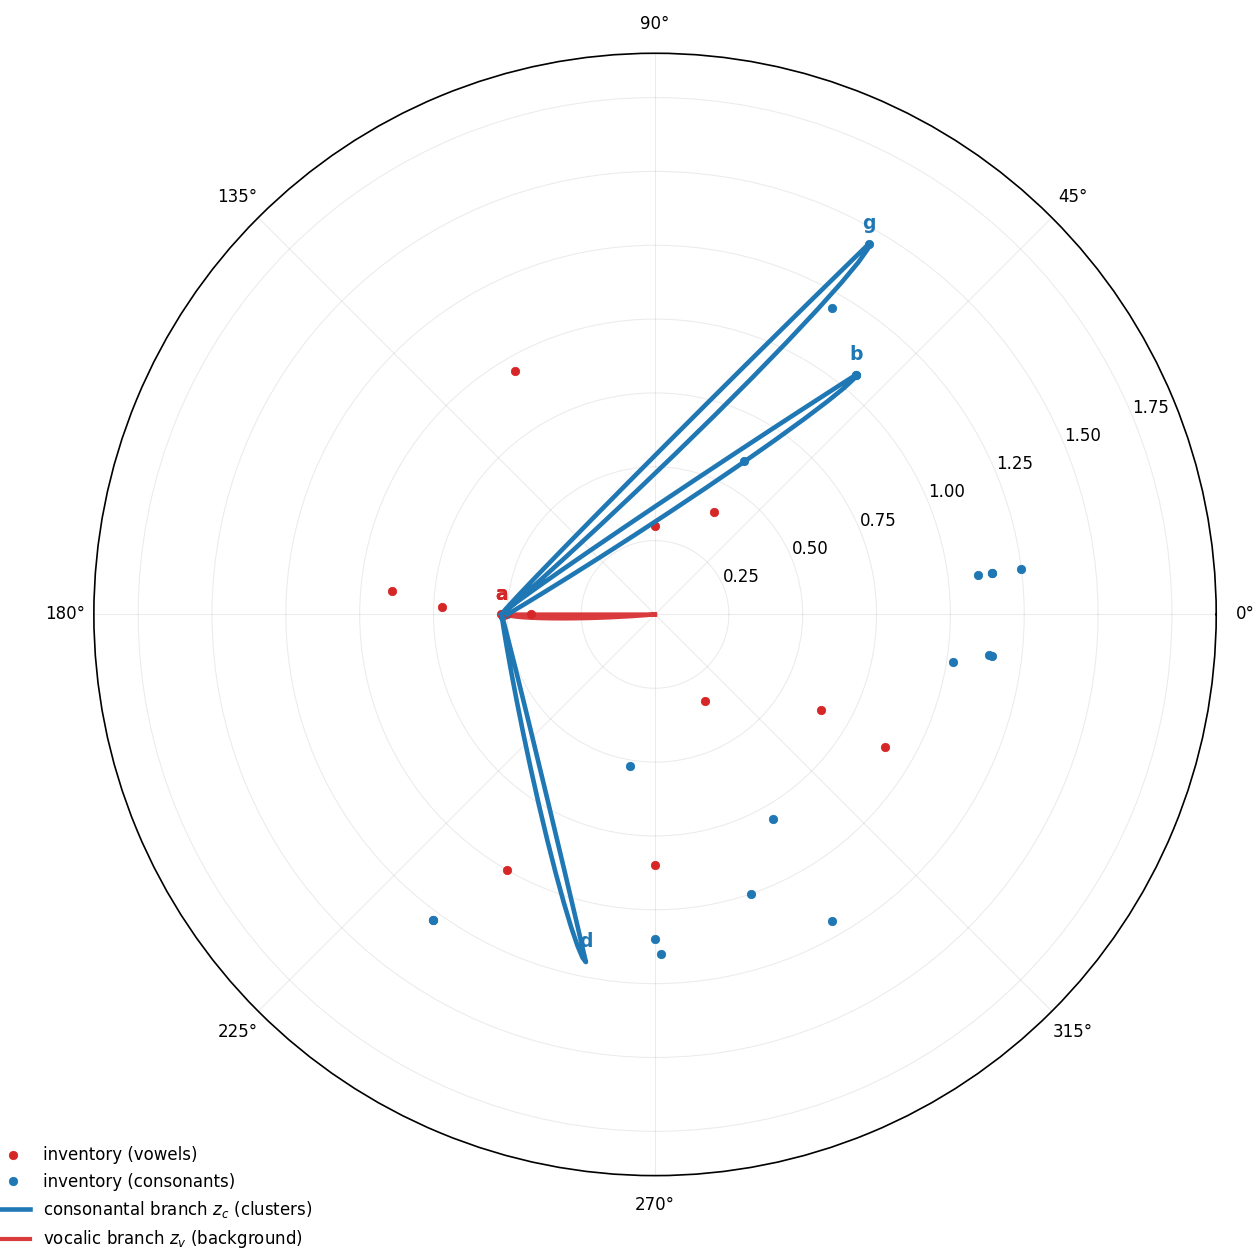
\includegraphics[width=0.62\textwidth]{figures/fig_branches_full.png}
\caption{Static view of the two branches for \code{ba.da.ga}
(JD3 speaker, internal notation). Red: the vocalic background
\vbranch, always active. Blue: the consonantal branch \cbranch,
active only during the three clusters; each blue excursion peaks
exactly on the consonant target (large dots: phoneme inventory;
small labels: phoneme keys at their targets).}
\label{fig:full}
\end{figure}

\subsection{Why two branches}

The displayed figure mirrors the synthesis architecture. Reconstructing
a single path by \emph{inverting} the 15 parameter frames actually
sent to the synthesizer (a least-squares fit of the polar projection)
cannot represent the superposition: inside a cluster the parameter
frames are a blend of two gestures and lie \emph{off} the polar
manifold, so the fit zigzags and the two branches collapse into one
visible path. The module therefore rebuilds both branches
\emph{directly from the engine's own polar points}, using the exact
arc machinery of the reference model
(Section~\ref{sec:reconstruction}). The inversion function
\code{polar\_from\_pval} is still shipped, as a diagnostic tool only.

% ===========================================================================
\section{The polar coordinate model}
% ===========================================================================

\subsection{Projection and targets}

The polar projection maps a target $(\rho, \theta)$ onto the
synthesizer parameter space. For every parameter $p$ of the 15
COVTL parameters, with calibration constants $c_0^{(p)}, c_1^{(p)},
c_2^{(p)}$ (columns of the matrix \code{CO}):

\begin{equation}
P_p(\rho, \theta) \;=\; c_1^{(p)} \;+\; \rho \, c_0^{(p)}
        \cos\!\bigl(c_2^{(p)} - \theta\bigr).
\label{eq:projection}
\end{equation}

Vowel targets come from the active speaker calibration
(\code{VOWEL\_TARGETS} in the installed constants, e.g.\ /a/ at
$\rho = 1.00$, $\theta = \pi$ on jd3/en); consonant targets from the consonant table plus contextual
place rules (dental /d/, velar /g/ resolved by vowel context,
cluster-specific adjustments). In the complex plane a target is the
complex number $z = \rho\, e^{i\theta}$.

\subsection{Arcs in the complex plane}

All motion is produced by one primitive, \code{polar.polar\_arc},
which interpolates between a departure point $z_1 = \rho_1
e^{i\theta_1}$ and an arrival point $z_2 = \rho_2 e^{i\theta_2}$.
Writing $\mathit{th}$ for a half-turn sweep from $0$ to $\pi$ (or
$\pi$ to $0$ when \code{orientation='inverse'}, which is the
departure-to-arrival direction used by the engine and the display)
and $r_k = \cos^2(\mathit{th}/2)$:

\begin{equation}
z(\mathit{th}) \;=\; \bigl(1 - r_k\bigr)\, z_1 \;+\;
      r_k \, \rho_2 \, e^{\,i\left(\theta_2 + \frac{\nu}{K}\,
      \mathit{th}\right)} .
\label{eq:arc}
\end{equation}

Three parameters control the shape of the path:

\begin{itemize}[leftmargin=1.4em]
\item \textbf{Curvature $K$.} The arrival angle carries an extra
      phase $\nu/K$; the smaller $K$, the more the arc bows away from
      the straight chord. The display uses
      $K = K_{\text{VOWEL\_DEFAULT}} = 30$ (Berthommier v15g
      reference), which gives a visible but moderate curvature
      (sagitta $2$--$2.4\,\%$ of the chord on the \code{ba.da.ga}
      validation corpus). Note that the trajectory \emph{engine}
      drives its parameter arcs with $K = 1000$ (quasi-rectilinear);
      using $K=30$ on screen is a deliberate visualization choice
      that restores the geometry of the reference model.
\item \textbf{Direction $\nu$.} $\nu = +1$ bows the vocalic arcs one
      way, $\nu = -1$ the consonantal sub-arcs the other way, as in
      the reference CV superposition figure.
\item \textbf{Angular path.} The arrival angle is unwrapped so the
      arc always takes the shortest angular route (no
      $-\pi \leftrightarrow +\pi$ wrap-around jumps).
\end{itemize}

Stationary holds (vowel plateaus, decay/attack anchors) are constant
complex samples produced by \code{polar.stationary\_point}. Both
primitives sample at $100$~Hz, the gesture rate of the engine
($1$ step $= 10$~ms).

\subsection{Superposition}

At every instant the final parameter frame sent to the synthesizer is
a blend: the \emph{selector} parameters owned by the active
consonants follow the consonantal branch, while all other parameters
follow the vocalic background (function
\code{build\_cluster\_pval} of \code{syltraj.py}). The figure
mirrors this architecture by keeping the two branches separate on
screen instead of merging them into one path.

% ===========================================================================
\section{From engine to figure: the two-branch reconstruction}
\label{sec:reconstruction}
% ===========================================================================

\subsection{Instrumented re-run of the engine}

The figure must show \emph{exactly} the timing of the synthesis. The
pipeline therefore re-runs the same engine function
(\code{syltraj.build\_phrase\_pval}, with the same normalization and
the same duration parameters) while temporarily wrapping the five
helpers of \code{build\_global\_pval} that carry the polar geometry.
Each helper records, per appended block and in
\code{block\_info} order, the polar points the engine drives toward:

\begin{center}
\begin{tabularx}{\textwidth}{@{}lX@{}}
\toprule
\textbf{Recorded event} & \textbf{Content} \\
\midrule
\code{arc} & departure and arrival anchor pair + duration in steps
(pause, initial and terminal arcs) \\
\code{bg} & anchor pair + duration (vocalic background arcs; the
schwa routing of closing VV arcs records its two half-arcs) \\
\code{hold} & anchor point + duration (decay/attack stationary
holds) \\
\code{cluster} & anchor pair, list of consonant \emph{node} targets
$[(\rho_k, \theta_k)]$ (context-adjusted), sub-arc duration $T$ \\
\bottomrule
\end{tabularx}
\end{center}

Vowel plateau blocks are appended inline by the engine (no helper to
wrap); the reconstruction rebuilds them from
\code{VOWEL\_TARGETS[vowel\_key]}. After the run, every queue must be
exactly consumed by a pass over \code{block\_info}; any leftover
event or duration mismatch raises a \code{RuntimeError} (alignment
drift guard), so a silent desynchronization of the figure with
respect to the audio is impossible by construction.

\subsection{Branch reconstruction rules}

The pass over \code{block\_info} emits, at 100~Hz, the two aligned
trajectories:

\begin{center}
\begin{tabularx}{\textwidth}{@{}>{\raggedright\arraybackslash}p{0.26\textwidth}X@{}}
\toprule
\textbf{Block kind} & \textbf{Branch behavior} \\
\midrule
plateau & red: stationary vowel target; blue: --- \\
background, pause, initial, terminal &
red: arc$(\mathit{dep}, \mathit{arr})$ with $K{=}30$, $\nu{=}{+}1$;
blue: --- \\
decay, attack & red: stationary anchor; blue: --- \\
cluster, $n = (m{+}1)\,T$ steps &
red: arc$(\mathit{dep}, \mathit{arr})$ over the whole block (the
background keeps flowing anchor to anchor); blue: sub-arcs
$\mathit{dep} \to C_1 \to \dots \to C_m \to \mathit{arr}$, $T$ steps
each, $K{=}30$, $\nu{=}{-}1$ \\
\bottomrule
\end{tabularx}
\end{center}

Two properties deserve emphasis. First, \emph{during a cluster the
red branch is not interrupted}: the vocalic background runs
underneath the consonant excursion (this is the \code{bg} component
of \code{build\_cluster\_pval}). Second, the blue branch peaks
\emph{exactly} on the consonant node targets at the end of each
approach sub-arc --- on the validation corpus \code{ba.da.ga} the
reconstructed peaks coincide with the engine targets to within
$10^{-9}$ (Table~\ref{tab:targets}).

\subsection{The .polar intermediate file (version 3)}

The result is stored in a self-documented JSON file with
\code{format}~=~\code{covtl-polar} and \code{version}~=~3:

\begin{lstlisting}[style=json]
{
  "format": "covtl-polar", "version": 3,
  "sample_rate": 100, "speaker": "JD3",
  "n_steps": 176, "duration_s": 1.76,
  "columns": { "vocalic_rho": "...", "consonantal_theta": "...", ... },
  "orientation": "trigonometric: theta=0 East, counter-clockwise",
  "trajectory": {
    "vocalic":     { "rho": [...], "theta": [...] },
    "consonantal": { "rho": [null, ..., 0.96, ...],   // null = inactive
                     "theta": [null, ..., 0.87, ...] }
  },
  "phonemes":  [ { "key": "b", "category": "C", "rho": 1.06,
                   "theta": 0.87, "t0": 20, "t1": 36 }, ... ],
  "inventory": [ { "key": "a", "category": "V", ... }, ... ]
}
\end{lstlisting}

The two 100~Hz trajectories are the single source of the figure ---
the video never re-derives them from the \code{.tract}. The
consonantal arrays carry \code{null} while the branch is inactive
(outside clusters), which lets the renderer break the blue curve
cleanly. Phoneme timing is in gesture steps ($10$~ms per step);
\code{t0}/\code{t1} are exact multiples of the block boundaries, so
the \code{.polar}, \code{.tract} and \code{.wav} timelines agree by
construction ($n_{\text{tract frames @400 Hz}} = 4 \times
n_{\text{steps}}$).

% ===========================================================================
\section{Rendering the figure}
% ===========================================================================

The final MP4 is a dual-panel composition at 25~Hz (H.264 + AAC,
audio muxed from the synthesized \code{.wav}):

\begin{itemize}[leftmargin=1.4em]
\item \textbf{Left panel}: the standard sagittal tract view, rendered
      from the \code{.tract} file (the standard video of the pipeline).
\item \textbf{Right panel}: the polar figure, in trigonometric
      orientation ($\theta = 0$ East, counter-clockwise), with:
      the two branch curves; a fading trail of $\approx 0.75$~s per
      branch (red and blue independently); a current-position dot
      per active branch; the phoneme inventory as small permanent
      dots (red vowels, blue consonants); a thin segment from the
      current position toward the active target; a transient label
      of the current phoneme (internal input notation, e.g.\ \code{tS},
      \code{a\textasciitilde}) displayed 0.5~s from the onset of the
      phoneme near its target.
\end{itemize}

\begin{figure}[ht]
\centering
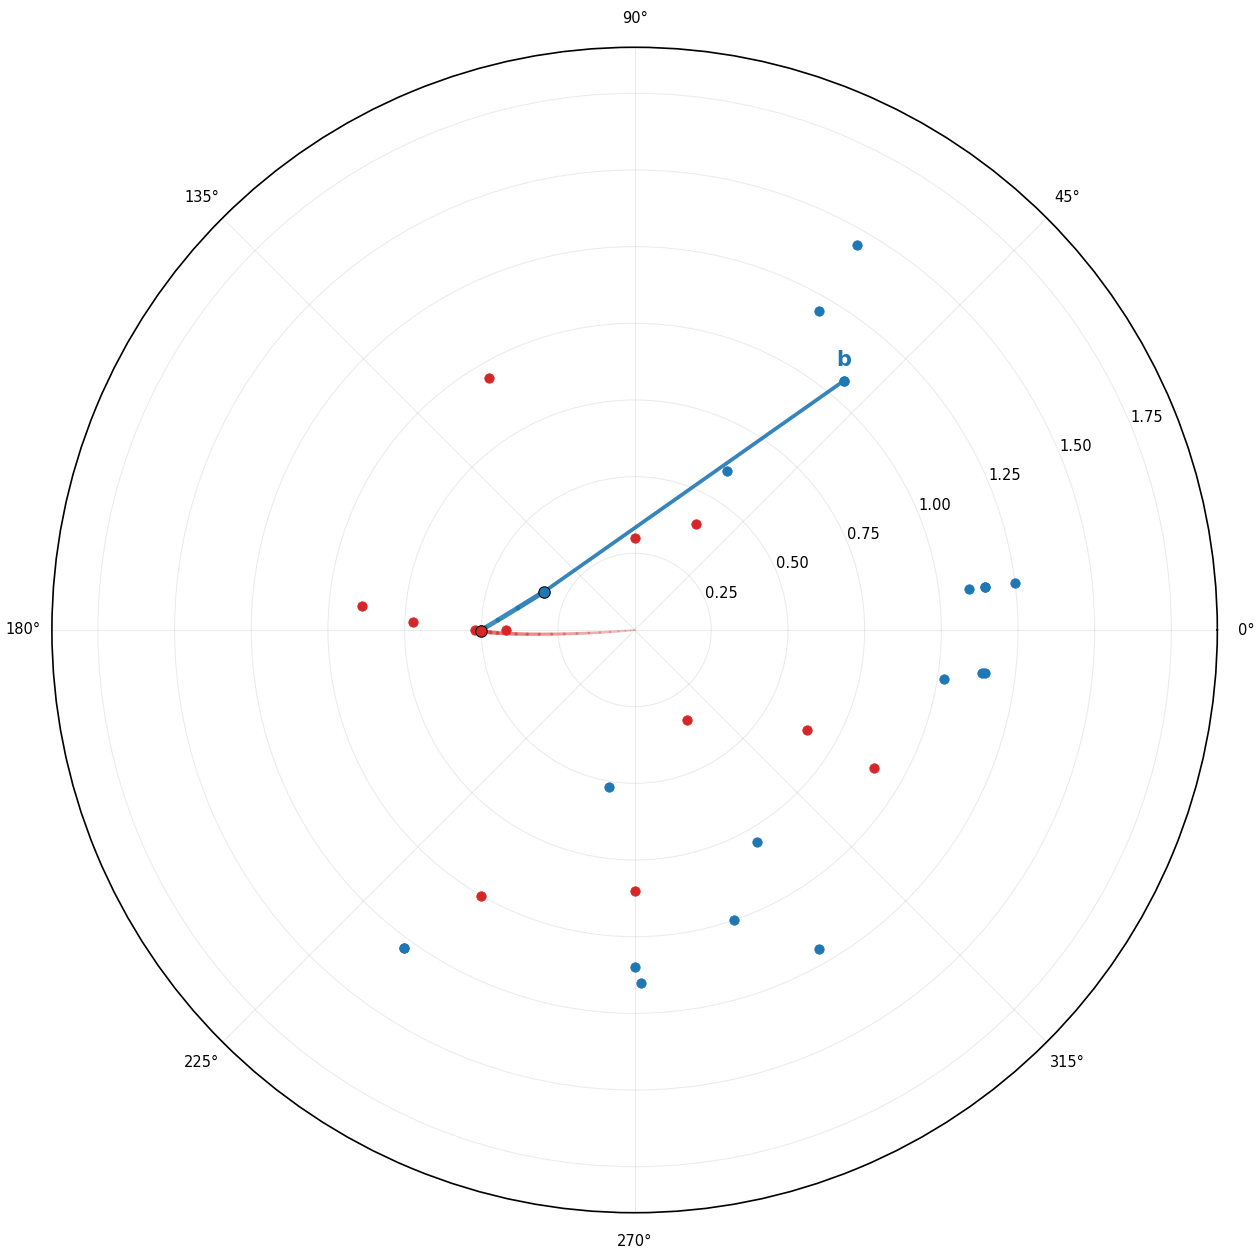
\includegraphics[width=0.58\textwidth]{figures/fig_frame_b.png}
\caption{Rendered frame at $t = 0.24$~s in \code{ba.da.ga}, during
the /b/ cluster: the blue branch has detached from the red background
and reaches the /b/ target (upper right, $\rho = 1.06$,
$\theta \approx 0.87$~rad), while the red background continues its
progression toward the vowel anchor.}
\label{fig:frameb}
\end{figure}

\begin{figure}[ht]
\centering
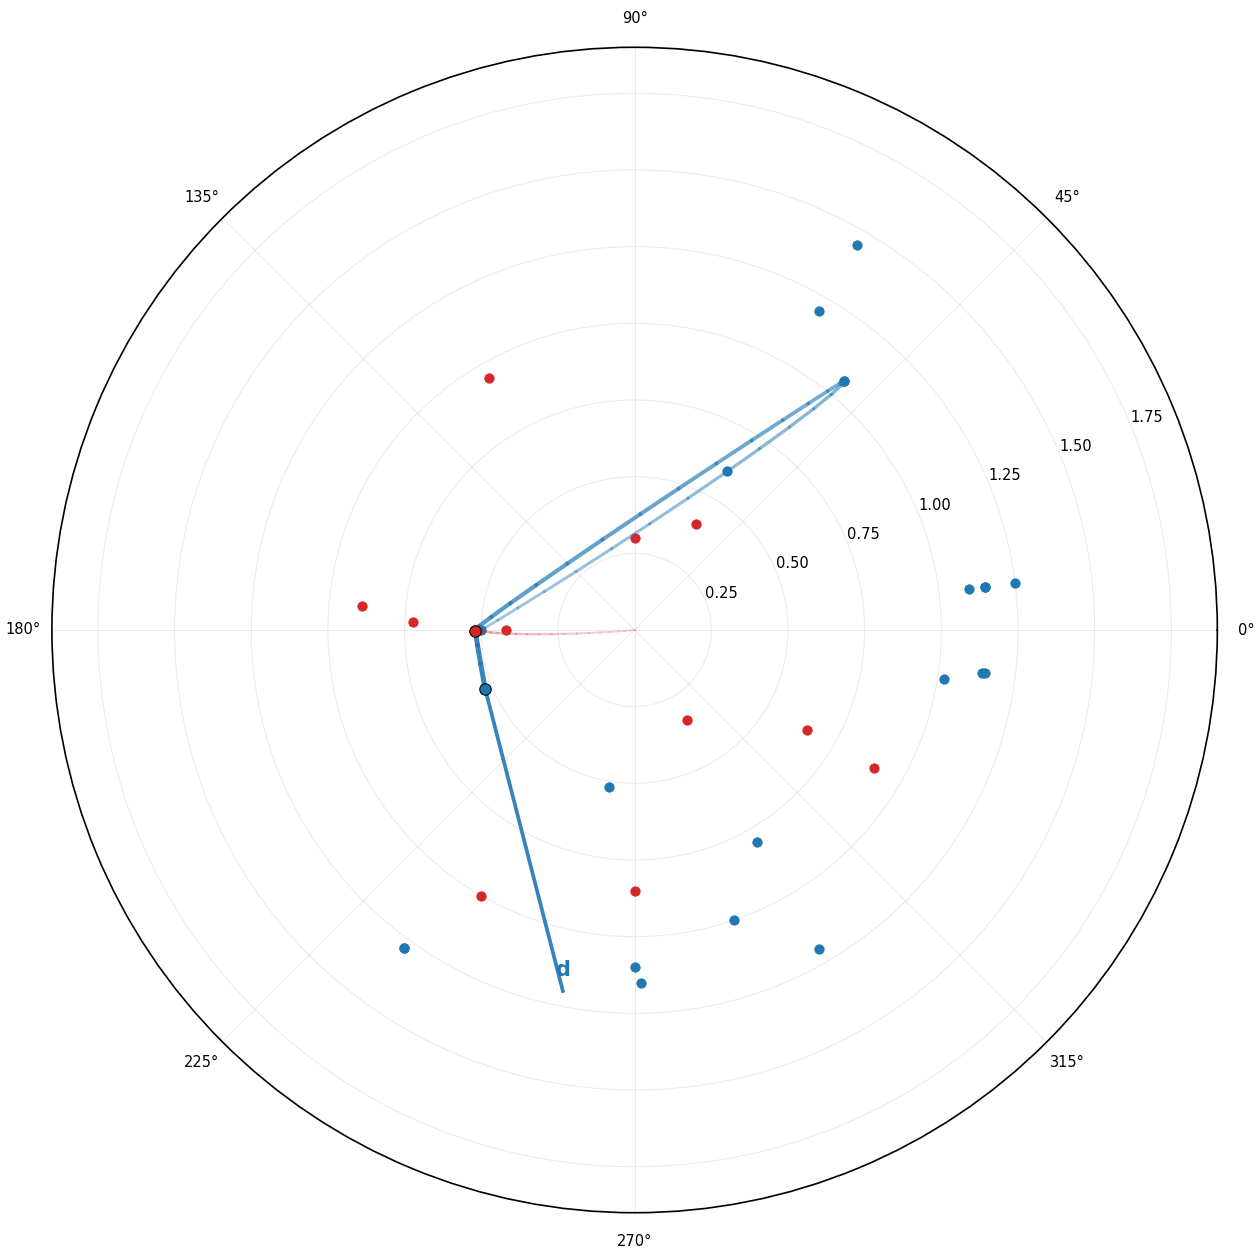
\includegraphics[width=0.58\textwidth]{figures/fig_frame_da.png}
\caption{Rendered frame at $t = 0.64$~s, during the /d/ cluster:
the fading blue trail of the /b/ excursion is still visible
(memory $\approx 0.75$~s) while a new blue excursion approaches the
/d/ target (bottom, $\rho = 1.2$, $\theta \approx -1.77$~rad);
the red background stays on the vowel axis. The two branches are
simultaneous and dissociated.}
\label{fig:frameda}
\end{figure}

% ===========================================================================
\section{Using the visualization}
% ===========================================================================

\subsection{Command line}

The feature is carried by three subcommands of \code{vtl-synth}; the
interfaces are identical to the rest of the pipeline:

\begin{lstlisting}[style=shell]
# Full chain: .tract + .wav + .polar + dual-panel .mp4
vtl-synth run --polar "this is easy for us" -l en -o out --label polar_demo_en

# .polar only, from a phrase in the internal notation
vtl-synth polar-build "ba.da.ga" -o out/ba.polar --tcons 160

# Dual-panel video from existing files
vtl-synth polar-video out/polar_demo_en.tract --polar out/polar_demo_en.polar \
        out/polar_demo_en.wav -o out/polar_demo_en.mp4
\end{lstlisting}

Reproducing the reference demos requires the \textbf{JD3 speaker} to
be the active speaker (\code{python install\_speaker.py install jd3};
restore your previous speaker afterwards). The engine options
(\code{-l}, \code{--tcons}, \code{--tvoy}, \code{--tpause},
\code{-f0}, \code{-s}) behave exactly as in \code{run} without
\code{--polar}, because the \code{.polar} build re-runs the same
engine with the same parameters.

\subsection{Python API}

\begin{lstlisting}[style=python]
from vtl_synth.video.polar_video import (
    build_polar, write_polar, read_polar,
    render_polar_frame, make_polar_video)

# 1. Build the two-branch trajectories (timings of the synthesis)
pol = build_polar(["ba.da.ga"], t_cons=16, t_voy=8,
                  pause_short_ms=200.0, pause_long_ms=320.0)
write_polar("out/ba.polar", pol)

# 2. Read it back
pol = read_polar("out/ba.polar")
zv, zc = pol["traj_v"], pol["traj_c"]   # (n, 2) rho/theta, NaN = inactive

# 3. Draw one frame (matplotlib polar axes) or the whole MP4
import matplotlib.pyplot as plt
fig = plt.figure(); ax = fig.add_subplot(111, projection="polar")
render_polar_frame(ax, pol, t=0.64)
make_polar_video("out/ba.tract", "out/ba.polar", wav_path="out/ba.wav",
                 out_path="out/ba.mp4")
\end{lstlisting}

% ===========================================================================
\section{Worked example and validation}
% ===========================================================================

The validation corpus is \code{ba.da.ga} with
$T_{\text{cons}} = 16$ steps (160~ms), $T_{\text{voy}} = 8$ steps,
pauses $200/320$~ms, JD3 speaker. Table~\ref{tab:targets} compares
the reconstructed blue-branch peaks with the engine consonant
targets; Figure~\ref{fig:full} (page~\pageref{fig:full}) shows the
full utterance.

\begin{table}[ht]
\centering
\caption{Blue-branch peaks vs.\ engine consonant targets on
\code{ba.da.ga} (JD3).}
\label{tab:targets}
\begin{tabular}{@{}lcccc@{}}
\toprule
\textbf{Consonant} & \textbf{Engine target} $(\rho, \theta)$ &
\textbf{Reconstructed peak} & \textbf{Error} &
\textbf{Sagitta ($\%$ chord)} \\
\midrule
/b/ & $(1.06,\ 0.87)$ & $(1.060,\ +0.873)$ & $<10^{-9}$ & $2.0$ \\
/d/ & $(1.20,\ -1.77)$ & $(1.200,\ -1.767)$ & $<10^{-9}$ & $2.4$ \\
/g/ & $(1.45,\ +1.05)$ & $(1.450,\ +1.047)$ & $<10^{-9}$ & $2.2$ \\
\bottomrule
\end{tabular}
\end{table}

Automated checks:

\begin{itemize}[leftmargin=1.4em]
\item \textbf{Targets.} every blue sub-arc terminates exactly on its
      node target (angle compared modulo $2\pi$).
\item \textbf{Simultaneity.} the blue branch is active on every step
      of each cluster block ($ (m{+}1)\,T$ steps: approach
      \emph{and} release), and only there.
\item \textbf{Background continuity.} the red branch is finite on
      every step of the utterance and rests exactly on the vowel
      target during plateaus.
\item \textbf{Curvature.} the sagitta of every sub-arc is between
      $2\,\%$ and $2.4\,\%$ of its chord ($K = 30$; the engine's
      $K = 1000$ would give $\approx 0.07\,\%$, invisible).
\item \textbf{Timeline.} \code{.polar} duration $=$ \code{.tract}
      duration $=$ MP4 duration (within one 25~Hz frame); the test
      selection \code{pytest tests -k "video or pipeline or cli or
      polar"} passes unchanged (9 tests).
\end{itemize}

% ===========================================================================
\section{Files, dependencies and demos}
% ===========================================================================

\subsection{Module and dependencies}

The feature is additive and self-contained: the synthesis path
(\code{core/polar.py}, \code{core/syltraj.py}) is only \emph{read}
(temporary instrumentation, restored in a \code{finally} block), so
the engine output and the regression baselines are untouched.
\code{Pipeline.run(...)} keeps its signature; the figure is activated
by the keyword \code{polar=True}, and the three CLI forms
(\code{run --polar}, \code{polar-build}, \code{polar-video}) reuse the
engine options (\code{-l}, \code{--tcons}, \code{--tvoy},
\code{--tpause}, \code{-f0}, \code{-s}) unchanged. The only
dependency is \code{matplotlib}, required by \code{run --polar}
(already listed for \code{plot-tract}):

\begin{lstlisting}[style=json]
[project.optional-dependencies]
plot  = ["matplotlib"]
video = ["Pillow", "imageio-ffmpeg", "matplotlib"]
\end{lstlisting}

\subsection{Files}

\begin{center}
\begin{tabularx}{\textwidth}{@{}lX@{}}
\toprule
\textbf{Path} & \textbf{Content} \\
\midrule
\code{vtl\_synth/video/polar\_video.py} & the polar-figure module
(build, read/write, frame rendering, dual-panel composition) \\
\code{docs/polar\_visualization.tex/.pdf} & this manual \\
\code{docs/figures/fig\_\*.png} & the figures of this manual \\
\code{examples/}, \code{out/} & showcase demos, regenerable (below) \\
\bottomrule
\end{tabularx}
\end{center}

The demo \emph{media} (\code{.mp4} $\approx$ 0.3--5~MB each, plus
\code{.tract}/\code{.wav}/\code{.polar}) may be committed as small
showcase files or regenerated on demand; prefer \textbf{Git LFS} for
the MP4s (\code{git lfs track "*.mp4"}).

\subsection{Regenerating the demos}

A minimal script regenerates the two showcase videos (JD3 must be the
active speaker, \code{python install\_speaker.py install jd3}; restore
the previous speaker afterwards):

\begin{lstlisting}[style=python]
from vtl_synth import Pipeline
for label, kwargs in [
    ("polar_demo_en", dict(text="this is easy for us", use_g2p=True)),
    ("polar_e2e", dict(text="ba.da.ga", use_g2p=False)),
]:
    Pipeline(f0_hz=102.216, speaker="JD3", t_cons_ms=100.0,
             t_voy_ms=80.0).run(
        kwargs["text"], output_dir="out", use_g2p=kwargs["use_g2p"],
        label=label, polar=True)
\end{lstlisting}

\subsection{Caveats}

\begin{itemize}[leftmargin=1.4em]
\item \textbf{Speaker dependence.} the figure uses the polar targets
      of the \emph{active} speaker constants. The reference demos are
      JD3; other speakers (s1, s2, m01, w02) work but their targets
      differ (e.g.\ /b/ is $(0.96, 4.90)$ for s2); see
      \code{docs/speakers.pdf}.
\item \textbf{Speaker switching.} generating the demos requires
      installing JD3 (\code{install\_speaker.py}), which swaps the
      shared wheel resource; restore the previous speaker afterwards.
\item \textbf{Display curvature.} $K = 30$ is a visualization
      constant (reference-model geometry); the parameter arcs of the
      engine remain $K = 1000$. This is intentional and documented in
      the module header.
\item \textbf{Work-directory hygiene.} the dual-panel encoder purges
      stale \code{frame\_*.png} files in its temporary work
      directories before rendering and verifies the composed frame
      count before encoding, so a video can never outlive its audio
      because of leftover frames of an earlier render.
\end{itemize}

\vspace{1.5em}
\begin{center}
\small\emph{Reference model: F.~Berthommier, ``COVTL'' technical
reports v15g, arXiv:2307.02299 (2023) and JEP 2024, pp.~541--550.}
\end{center}

\end{document}
